\documentclass{article}
\usepackage{parskip}
\usepackage{graphicx}
\usepackage{amsmath}
\usepackage[margin=.6in]{geometry}
\begin{document}

\title{Computer Security and Privacy Assignment 3}
\date{July 26, 2016}
\author{Lariesa Janecka, lajaneck, 20460089}
\maketitle


\section*{Question 1}
\label{sec:question_1}
\subsection*{a)}
\label{sub:a_}
The world interacts with a surface router. This router directs packets  to an internal router which redirects those packets to the closest geographic location. At this location there is a webserver, database, and file server. The webserver just serves the user interface for the website. The file server is attached to the database to authenticate the user's credentials and if they have access to the content that they have requested. This way the webserver can authenticate the user with access to the database, but databases and file servers have redundancy by residing at each geographical location.

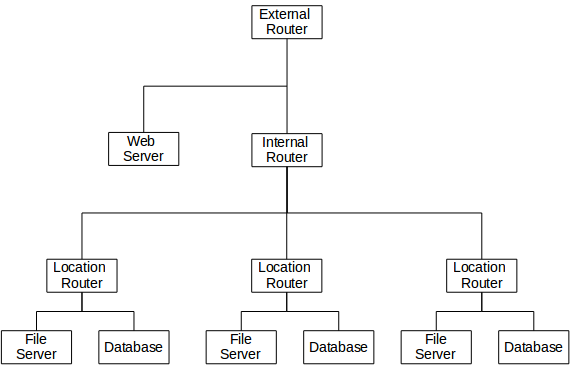
\includegraphics[scale=0.8]{network}

\subsection*{b)}
\label{sub:b_}
The firewall should go right before the internal router. this way the webserver can sit in the demilitarized zone and not be slowed down by the firewall. Users will see their interface as responsive and possible. A this location the firewall can still filter packets to all sensitive locations even though we only have one firewall.

This firewall should be a simple packet filtering gate way. This is because little is known about the packet's final destination application so an application proxy won't work. Literally every packet served by the application will go through this firewall so it is important that it be as fast as possible because any cost will have massive repercussions so a stateful firewall will cost too much. Because of this only a simple packet filtering firewall will do.

\subsection*{c)}
\label{sub:c_}
If we have a firewall for each geographical location we can put a more specific firewall at the nexus for each of those locations (right before traffic divides into database and fileserver requests). This firewall can be stateful because a much smaller subset of traffic is going through here. We could even use an application firewall with configurations for database access and file server accesses.

\section*{Question 2}
\label{sec:question_2}
\subsection*{a)}
\label{sub:a_}
\paragraph{Assumption}
\label{par:assumption}
This attack assumes that usernames are evenly distributed across the alphabet (i.e. there are the same number of usernames starting with a as there are starting with x).
\paragraph{Tracker}
\label{par:tracker}
Get roughly half the usernames, this works out to be usernames greater than m. This relies on the above stated assumption since this wouldn't work if every username started with x. Since $k = \frac{N}{8}$ we can easily see that $2 \frac{N}{8} < \frac{N}{2} < N - 2 \frac{N}{8}$
\paragraph{Queries}
\label{par:queries}
\begin{itemize}
	\item $username == XdarksephirothX || username > m$
	\item $username != XdarksephirothX \&\& username \leq m$
	\item true
\end{itemize}
\subsection*{b)}
\label{sub:b_}
First run the query $username < m$. This gives us a baseline to work with. Then we can run $username < m || (username == XdarksephirothX \&\& gold <= x)$ and watch for when the value returned is one greater than the established base line. You can now narrow down on the correct value of x using a binary search within the bounds of zero and 20 billion.  This should always return roughly half or half plus one values (again, assuming that names are evenly distributed) so we get around the restrictions on queries. 

\section*{Question 3}
\label{sec:question_3}
\subsection*{a)}
\label{sub:a_}
The first major issue is that it is often very hard to determine which district a hacker's computer resides, so law enforcers cannot tell which judge should sign the warrant. This makes getting warrants and prosecuting these criminals much harder. With these changes the police just have to get a warrant from the nearest judge without having to know the physical location of the hacker. 

The second issue is that many hackers use bot nets which include thousands of devices in many different districts. Thats a lot of warrants from a lot of different judges. With these bill changes only one warrant (and by extension one judge) are required to shut down bot nets.
\subsection*{b)}
\label{sub:b_}
Peter Carr is referring to how crazy good hackers are at hiding their identity and location. Without knowledge of who to serve the warrant to and which district needs to approve of it, it is impossible to get a warrant. 
\subsection*{c)}
\label{sub:c_}
The government could freely hack anyone who has ever torrented (or any form of peer to peer sharing) anything. Dropbox (and similar services) would also be wrecked. If any user uploads copyrighted content to their dropbox the government now has the ability to hack Dropbox (from there they can access everyone who has copyrighted content on their dropbox). VPNs would also be hit pretty hard because one bad apple could get then entire network hacked by the police.
\subsection*{d)}
\label{sub:d_}
This policy change could allow investigators to search many different computers with a single warrant, including computers of people who were just victims and didn't even know they were involved. It would also allow judges to approve of warrants in districts that are not their own, allowing investigators to chose the judge they ask.
\subsection*{e)}
\label{sub:e_}
Judge shopping is filling a bunch of stuff in various locations and hoping that one of the many different judges is sympathetic. An example of this would be if you petitioned a judge for a warrant and if you're rejected going to a different judge by claiming your warrant is somehow related to something in their district so they might sign it.



\section*{Programming Questions}
\label{sec:programming_questions}
\subsection*{Question 1}
\label{sub:question_1}
The worst case is $NbW$ and the average case is $NbW/2$

\subsection*{Question 2}
\label{sub:question_2}
You could introduce signing to your packets being sent for decryption which would ensure that the person sending the cipher text is the one that did the encrypting. This would provide authentication. The attacker needs to be able to get the server to check the padding of the text, but if we sign our packets then the attacker can't get a response. 

\subsection*{Question 3}
\label{sub:question_3}
For section* 3.1 we need to change line 5b to xor using n-1, n-2, ..., 1 and line 6 to xor with n in order to match our current padding scheme.

For section* 3.2 we need to change line 1 to xor with the correct values to match our new padding scheme instead of one consistent value as matches with the previous padding scheme.










\end{document}	